\documentclass{article}
\usepackage[utf8]{inputenc}
\usepackage{indentfirst}
\usepackage{titling}
\usepackage{geometry}
\usepackage{graphicx}
\graphicspath{ {./Images/} }
\usepackage[shortlabels]{enumitem}
\usepackage{fancyhdr}
\usepackage{ulem}
\usepackage[dvipsnames]{xcolor}
\usepackage{amssymb}

\def\ojoin{\setbox0=\hbox{$\bowtie$}%
  \rule[-.02ex]{.25em}{.4pt}\llap{\rule[\ht0]{.25em}{.4pt}}}
\def\leftouterjoin{\mathbin{\ojoin\mkern-5.8mu\bowtie}}
\def\rightouterjoin{\mathbin{\bowtie\mkern-5.8mu\ojoin}}
\def\fullouterjoin{\mathbin{\ojoin\mkern-5.8mu\bowtie\mkern-5.8mu\ojoin}}

\renewcommand\maketitlehooka{\null\mbox{}\vfill} %para centralizar verticalmente
\renewcommand\maketitlehookd{\vfill\null}
\pagestyle{fancy}
\fancyhf{}
\rfoot{\thepage}
\lfoot{ 
\includegraphics[scale=0.01]{UA.jpg} José Mendes 107188 LEI}
\geometry{
  a4paper,
  headheight=4cm,
  top=5.5cm,
  bottom=4.5cm,
  footskip=4cm
}


\title{Complementos de Bases de Dados}
\author{José Mendes 107188}
\date{2023}

\begin{document}


\begin{titlepage}
    \maketitle
    \begin{center}
        
\includegraphics[scale=0.4]{UA.png}
    \end{center}
    \thispagestyle{empty} %remove o count da pagina
\end{titlepage}

\pagebreak
%depois por um index aqui

\section{Evolução dos Sistemas de Base de Dados}

\begin{flushleft}
    \textbf{Sistemas de Dados -} Cada vez mais as aplicações de hoje em dia
    são Data-Intensive, em vez de Compute-Intensive. 

    Para Data-Intensive, o poder bruto da CPU deixa de ser um fator limitante
    quando comparado com a \textbf{quantidade}, \textbf{complexidade} e \textbf{velocidade de atualização} dos dados.

    \vspace{3mm}

    De forma a otimizar a sua performance, um sistema de dados tipicamente oferece as seguintes
    funcionalidades:
    \begin{enumerate}
      \item \textbf{Bases de Dados -} armazenam os dados para utilização futura;
      \item \textbf{Caches -} guardam os resultados de operações dispendiosas, de forma a tornar a leitura mais rápida;
      \item \textbf{Search Indexes -} permitem aos utilizadores procurarem por palavras-chave ou filtrar os dados;
      \item \textbf{Message Queues -} permitem a comunicação assíncrona entre processos;
      \item \textbf{Stream Processing -} permite o processamento de dados em tempo real;
      \item \textbf{Batch Processing -} permite o processamento de dados acumulados, periodicamente;
    \end{enumerate}

    \textcolor{Blue}{Exemplo:}
    Um exemplo de \textbf{stream processing} ocorre na banca. Sempre que é realizada uma transação, os dados da mesma são
  imediatamente processados de forma a que o saldo esteja sempre atualizado.


  O \textbf{batch processing} é visível na faturação dos serviços pós-pagos pelas operadoras de telecomunicações. No final de
  cada mês, é feita uma consulta às suas bases de dados de forma a identificar todos os consumos do cliente, que são
  somados e depois gerada a fatura.


  No \textbf{stream} os dados são processados antes de armazenados, enquanto que no \textbf{batch} são processados depois de
  armazenados.

  \vspace{3mm}

  Cada vez mais as aplicações requerem um \textbf{maior wide-range de requisitos}. Muitas das vezes,
  \uline{uma única ferramenta já não consegue satisfazer todas as necessidades de \textbf{data processing} e \textbf{storage}}.

  \vspace{2mm}

  Em vez disso, o \uline{trabalho é partido em tasks que possam ser realizadas de forma eficiente
  por uma única ferramenta}. As ferramentas individuais utilizadas são depois juntas utilizando
  código de aplicação.

  \vspace{2mm}

  \textcolor{Blue}{Exemplo:} Podemos ter uma aplicação que utiliza uma Catching Layer (\textbf{memcached}), um Full-Text Search (\textbf{Elasticsearch})
  e uma Base de Dados principal separada (\textbf{MySQL}).
\end{flushleft}

\begin{center}
  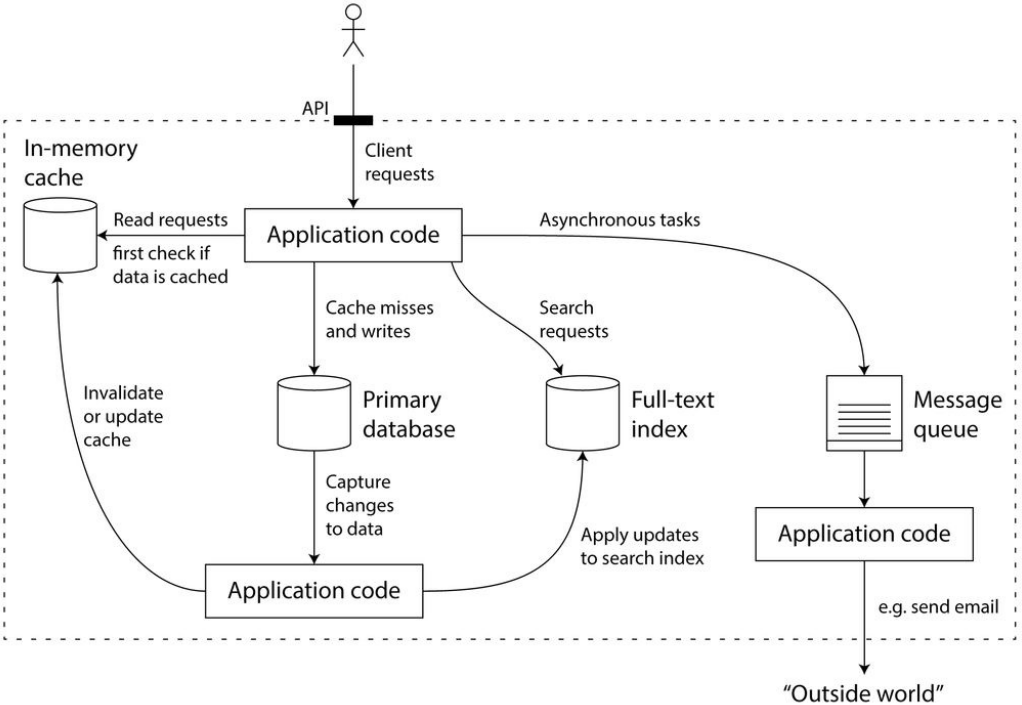
\includegraphics[scale=0.3]{1.png}
\end{center}

\subsection{Desafios que os Sistemas de Dados enfrentam}

\begin{flushleft}
  \item Como garantir que todos os dados se mantêm corretos e consistentes, mesmo quando, internamente, ocorreu algum erro? (ex: persistência de dados)
  \item Como fornecer boa performance para os clientes, mesmo quando partes do sistema estão degredadas?
  \item Como escalar o sistema para ser capaz de aguentar uma load intensiva de trabalho?
  \item Qual a aparência de uma boa API para o serviço?
\end{flushleft}

\subsection{Alguns Requisitos}

\begin{flushleft}
  \item \textbf{Fiabilidade -} O Sistema deve continuar a funcionar corretamente em caso de adversidades (ex: falhas de hardware, software ou mesmo humanas).
  \item \textbf{Escalabilidade -} O Sistema deve ser capaz de responder ao crescimento seja do volume de dados, do tráfego, ou mesmo da complexidade.
  \item \textbf{Manutenibilidade -} Deve ser possível que o Sistema sofra alterações ao longo do tempo por várias pessoas diferentes de forma produtiva.
\end{flushleft}

\pagebreak

\subsection{Bases de Dados}

\begin{flushleft}
  São definidas como um \uline{conjunto de dados relacionados entre si e a sua organização}.
  \vspace{2mm}
  Dividem-se em vários tipos, sendo atualmente os mais comuns: \textbf{Relacionais}, seguidas por
  \textbf{Documentais}, \textbf{Motores de busca}, \textbf{Chave-Valor}, entre outras. 
  \vspace{2mm}
  O controlo às bases de dados é realizado por \textbf{Sistemas de Gestão de Base de Dados} (\textbf{SGBD}
  ou DBMS em inglês). Estes fornecem funções que permitem a manipulação de grandes
  quantidades de informação.
\end{flushleft}



\vspace{3mm}






\end{document}